\documentclass[11pt]{article}

% packages
\usepackage{physics}
% margin spacing
\usepackage[top=1in, bottom=1in, left=0.5in, right=0.5in]{geometry}
\usepackage{hanging}
\usepackage{amsfonts, amsmath, amssymb}
\usepackage[none]{hyphenat}
\usepackage{fancyhdr}
\usepackage[nottoc, notlot, notlof]{tocbibind}
\usepackage{graphicx}
\graphicspath{{./images/}}
\usepackage{float}
\usepackage{siunitx}
\usepackage{esint}
\usepackage{cancel}

% header/footer formatting
\pagestyle{fancy}
\fancyhead{}
\fancyfoot{}
% define a new page style called firststyle
\fancyhead[L]{Invariance of Green's theorem under coordinate changes}
\fancyhead[R]{Sai Sivakumar}
\fancyfoot[R]{\thepage}
\renewcommand{\headrulewidth}{0pt}

% paragraph indentation/spacing
\setlength{\parindent}{0cm}
\setlength{\parskip}{5pt}
\renewcommand{\baselinestretch}{1.25}

% extra commands defined here
\newcommand{\ihat}{\boldsymbol{\hat{\textbf{\i}}}}
\newcommand{\jhat}{\boldsymbol{\hat{\textbf{\j}}}}
\newcommand{\dr}{\vec{r}~^{\prime}(t)}
\newcommand{\dx}{x^{\prime}(t)}
\newcommand{\dy}{y^{\prime}(t)}

\newcommand{\br}[1]{\left(#1\right)}
\newcommand{\sbr}[1]{\left[#1\right]}
\newcommand{\cbr}[1]{\{#1\}}

\newcommand{\dprime}{\prime\prime}
\newcommand{\lap}[2]{\mathcal{L}[#1](#2)}

% bracket notation for inner product
\usepackage{mathtools}

\DeclarePairedDelimiterX{\abr}[1]{\langle}{\rangle}{#1}

% set page count index to begin from 1
\setcounter{page}{1}

\begin{document}

Show that the formula in Green's theorem is invariant under coordinate changes, in the sense that if the theorem holds for a bounded domain $U$ with piecewise smooth boundary, and if $F(x,y)$ is a smooth function that maps $U$ one-to-one onto another such domain $V$ and that maps the boundary of $U$ one-to-one smoothly onto the boundary of $V$, then Green's theorem holds for $V$. \textit{Hint}. First note the change of variable formulae for line and area integrals, given by
\begin{align*}
    \int_{\partial V}P\dd{\xi} &= \int_{\partial U}\br{P\circ F}\br{\pdv{\xi}{x}\dd{x} + \pdv{\xi}{y}\dd{y}}\\
    \iint_V R\dd{\xi}\dd{\eta} &= \iint_U \br{R\circ F}\det J_F\dd{x}\dd{y}
\end{align*}
where $F:\mathbb{R}^2\to \mathbb{R}^2$ is the transformation $(x,y)\to (\xi(x,y),\eta(x,y))$, and where $J_F$ is the Jacobian matrix of $F$ (take the absolute value of the determinant). Use these formulae, with $R=-\pdv{P}{\eta}$. The summand $\int_{\partial V} Q\dd{\eta}$ is treated similarly.

%\begin{figure}[h]
%    \centering
%    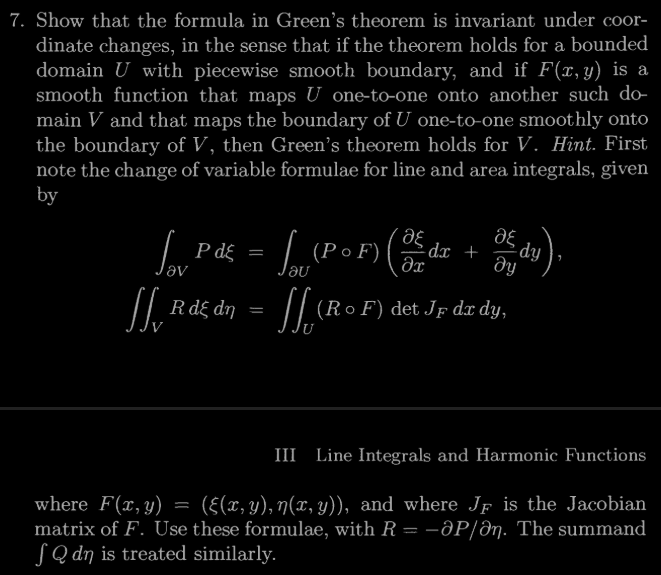
\includegraphics[scale=0.5]{problem}
%\end{figure}

All the conditions are met for Green's theorem. Then generically the formula we know for Green's theorem is:
$$\int_{\partial D} P\dd{x} + Q\dd{y} = \iint_D \br{Q^{\prime}_x - P^{\prime}_y}\dd{x}\dd{y}$$

Start with the following change of variables (after which $\xi$ and $\eta$ are read as functions of $(x,y)$):
\begin{align*}
    \int_{\partial V} P\dd{\xi} + Q\dd{\eta} &= \int_{\partial U} \br{P\circ F}\br{\xi^{\prime}_x\dd{x} + \xi^{\prime}_y\dd{y}} + \br{Q\circ F}\br{\eta^{\prime}_x\dd{x} + \eta^{\prime}_y\dd{y}} \\
    &= \int_{\partial U}\br{\br{P\circ F}\xi^{\prime}_x + \br{Q\circ F}\eta^{\prime}_x}\dd{x} + \br{\br{P\circ F}\xi^{\prime}_y + \br{Q\circ F}\eta^{\prime}_y}\dd{y}
\end{align*}

Then apply Green's theorem:
%$$\int_{\partial U}\br{\br{P\circ F}\xi^{\prime}_x + \br{Q\circ F}\eta^{\prime}_x}\dd{x} + \br{\br{P\circ F}\xi^{\prime}_y + \br{Q\circ F}\eta^{\prime}_y}\dd{y}$$
\begin{align*}
    &= \iint_U\sbr{ \dv{x}\br{\br{P\circ F}\xi^{\prime}_y + \br{Q\circ F}\eta^{\prime}_y} - \dv{y}\br{\br{P\circ F}\xi^{\prime}_x + \br{Q\circ F}\eta^{\prime}_x} }\dd{x}\dd{y}\\
    &= \iint_U\bigg[\dv{\br{P\circ F}}{x}\xi^{\prime}_y + \br{P\circ F}\xi^{\dprime}_{yx} + \dv{\br{Q\circ F}}{x}\eta^{\prime}_y + \br{Q\circ F}\eta^{\dprime}_{yx} \\ &~~~~ - \dv{\br{P\circ F}}{y}\xi^{\prime}_x - \br{P\circ F}\xi^{\dprime}_{xy} - \dv{\br{Q\circ F}}{y}\eta^{\prime}_x - \br{Q\circ F}\eta^{\dprime}_{xy}\bigg]\dd{x}\dd{y}
\end{align*}

Cancel out the terms containing mixed second partial derivatives via Clairaut's theorem. Continue by using the chain rule, and for brevity, let $\mathcal{P} = P\circ F$ and $\mathcal{Q} = Q\circ F$:
\begin{align*}
    &= \iint_U\sbr{\dv{\br{P\circ F}}{x}\xi^{\prime}_y + \dv{\br{Q\circ F}}{x}\eta^{\prime}_y - \dv{\br{P\circ F}}{y}\xi^{\prime}_x - \dv{\br{Q\circ F}}{y}\eta^{\prime}_x }\dd{x}\dd{y} \\
    &= \iint_U \sbr{\mathcal{P}^{\prime}_{\xi}\xi^{\prime}_{x}\xi^{\prime}_{y} + \mathcal{P}^{\prime}_{\eta}\eta^{\prime}_{x}\xi^{\prime}_{y} + \mathcal{Q}^{\prime}_{\xi}\xi^{\prime}_{x}\eta^{\prime}_{y} + \mathcal{Q}^{\prime}_{\eta}\eta^{\prime}_{x}\eta^{\prime}_{y} - \mathcal{P}^{\prime}_{\xi}\xi^{\prime}_{y}\xi^{\prime}_{x} - \mathcal{P}^{\prime}_{\eta}\eta^{\prime}_{y}\xi^{\prime}_{x} - \mathcal{Q}^{\prime}_{\xi}\xi^{\prime}_{y}\eta^{\prime}_{x} - \mathcal{Q}^{\prime}_{\eta}\eta^{\prime}_{y}\eta^{\prime}_{x}}\dd{x}\dd{y} \\
    &= \iint_U \sbr{\mathcal{P}^{\prime}_{\eta}\eta^{\prime}_{x}\xi^{\prime}_{y} + \mathcal{Q}^{\prime}_{\xi}\xi^{\prime}_{x}\eta^{\prime}_{y} - \mathcal{P}^{\prime}_{\eta}\eta^{\prime}_{y}\xi^{\prime}_{x} - \mathcal{Q}^{\prime}_{\xi}\xi^{\prime}_{y}\eta^{\prime}_{x}}\dd{x}\dd{y} \\
    &= \iint_U \br{\mathcal{Q}^{\prime}_{\xi} - \mathcal{P}^{\prime}_{\eta}}\det J_F\dd{x}\dd{y} \\
\end{align*}

Carry out the change of variables for area integrals to find the result we want:
\begin{align*}
    \iint_U \br{\mathcal{Q}^{\prime}_{\xi} - \mathcal{P}^{\prime}_{\eta}}\det J_F\dd{x}\dd{y} &= \iint_V \br{Q^{\prime}_{\xi} - P^{\prime}_{\eta}}\dd{\xi}\dd{\eta}
\end{align*}

Hence Green's theorem holds for $V$:
$$\int_{\partial V} P\dd{\xi} + Q\dd{\eta} = \iint_V \br{Q^{\prime}_{\xi} - P^{\prime}_{\eta}}\dd{\xi}\dd{\eta}$$

\end{document}